\documentclass[a4j,12pt]{jreport}
\makeatletter
\usepackage{url}
\usepackage{jtygm}
\usepackage{ascmac}
\usepackage[dvipdfmx]{graphicx}
\usepackage{amsmath,amssymb}
\usepackage{multicol}
\usepackage{listings}
\usepackage{makeidx}
\usepackage{ccaption}
\usepackage{here}
\usepackage{subfigure}
\usepackage{enumerate}
\usepackage[dvipdfmx]{color}
\usepackage{fancybox}
\usepackage{geometry}
\usepackage{ascmac}
\usepackage{titletoc}
\usepackage{titlesec}
\usepackage{framed}
\usepackage{longtable}
\usepackage{ulem}
\usepackage{anyfontsize}
\usepackage{wrapfig}
\usepackage{bm}

\renewcommand{\lstlistingname}{リスト}

\newcommand{\minisec}[1]{
\subsubsection{【#1】}
}

\geometry{
body={384pt,574pt},
hmargin={2.0cm,2.0cm},
vmargin={2.5cm,2.0cm},
bindingoffset=0.5cm,
twoside
}

% 付録の始まり
\newcommand{\beginappendix}{
  % 章番号の書式変更
  \setcounter{chapter}{0}
  \renewcommand{\prechaptername}{付録}
  \renewcommand{\postchaptername}{} 
  \renewcommand{\thechapter}{\@Alph\c@chapter}
  \renewcommand{\thesection}{\@Alph\c@chapter.\@arabic\c@section}
  \renewcommand{\thesubsection}{\@Alph\c@chapter.\@arabic\c@section.\@arabic\c@subsection}
}

%図番号の書式変更
  \renewcommand{\thefigure}{%
  \thechapter.\arabic{figure}}
  \@addtoreset{figure}{chapter}
\makeatother


\newcommand{\ruby}[2]{%
\leavevmode
\setbox0=\hbox{#1}%
\setbox1=\hbox{\tiny #2}%
\ifdim\wd0>\wd1 \dimen0=\wd0 \else \dimen0=\wd1 \fi
\hbox{%
\kanjiskip=0pt plus 2fil
\xkanjiskip=0pt plus 2fil
\vbox{%
\hbox to \dimen0{%
\tiny \hfil#2\hfil}%
\nointerlineskip
\hbox to \dimen0{\mathstrut\hfil#1\hfil}}}}

\makeatletter
\lstset{% 
language={C}, 
frame=trbl,% 
basicstyle={\small},% 
identifierstyle={\small},% 
commentstyle={\small\ttfamily},% 
keywordstyle={\small\bfseries},% 
ndkeywordstyle={\small},% 
stringstyle={\small\ttfamily}, 
tabsize=2,
breaklines=true, 
frame=none,
columns=[l]{fullflexible},% 
numbers=left,% 
xrightmargin=0zw,% 
xleftmargin=3zw,% 
numberstyle={\scriptsize},% 
stepnumber=1, 
numbersep=1zw,% 
backgroundcolor={\color[gray]{.90}},
} 

%footnoteにおいてverbを有効にする設定
\long\def\@footnotetext{%
  \insert\footins\bgroup
    \normalfont\footnotesize
    \interlinepenalty\interfootnotelinepenalty
    \splittopskip\footnotesep
    \splitmaxdepth \dp\strutbox \floatingpenalty \@MM
    \hsize\columnwidth \@parboxrestore
    \protected@edef\@currentlabel{%
       \csname p@footnote\endcsname\@thefnmark
    }%
    \color@begingroup
      \@makefntext{%
        \rule\z@\footnotesep\ignorespaces}%
      \futurelet\next\fo@t}
\def\fo@t{\ifcat\bgroup\noexpand\next \let\next\f@@t
                                \else \let\next\f@t\fi \next}
\def\fo@t{\bgroup\aftergroup\@foot\let\next}
\def\f@t#1{#1\@foot}
\def\@foot{\@finalstrut\strutbox\color@endgroup\egroup}

\renewcommand{\seename}{→}
\makeatother

%-----目次及び見出し-----
\contentsmargin{0pt}
  \titlecontents{chapter}[5.6pc]
  {\addvspace{10pt}\bfseries}
  {\contentslabel[\thecontentslabel]{4.6pc}}
  {}
  {\hfill\normalfont\thecontentspage}

  \titlecontents{section}[4.8pc]
  {\addvspace{4pt}\bfseries}
  {\contentslabel[\thecontentslabel]{2.8pc}}
  {}
  {\dotfill\thecontentspage}

  \titlecontents{subsection}[6.4pc]
  {\addvspace{2pt} }
  {\contentslabel[\thecontentslabel]{3.4pc}}
  {}
  {\dotfill\normalfont \thecontentspage }

 \titleformat{\chapter}[frame]
  {\small}
  {\filright
   \large
  第 \thechapter 章}
  {8pt}
  {\LARGE\bfseries\filcenter}

\titleformat{\section}[hang]{\large\bfseries}
{\colorbox{black}{\color{white}\thesection}}{12pt}{}%
[{\titlerule[1pt]}]

\titleformat{\subsection}[block]
{\normalfont\bfseries}{\fbox{\itshape\thesubsection}}{1em}{}
[{\titlerule[0.5pt]}]

 \titlespacing{\chapter}{0pt}{4pt plus 2pt minus 1pt}{2pt plus 2pt minus 2pt}
 \titlespacing{\section}{0pt}{0pt plus 0pt minus 0pt}{0pt plus 0pt minus 0pt}
 \titlespacing{\subsection}{0pt}{0pt plus 0pt minus 0pt}{0pt plus 0pt minus 0pt}
\newenvironment{code}{
\VerbatimEnvironment
\begin{quote}
\begin{Verbatim}	
}
{
\end{Verbatim}
\end{quote}
}

\newenvironment{problems}
{
  \renewcommand\labelenumi{\doublebox{\arabic{enumi}}}
  \begin{enumerate}
}{
  \end{enumerate}
  \renewcommand\labelenumi{\arabic{enumi}.}
}


\makeindex

\begin{document}
\makeatletter
\renewcommand{\thelstlisting}{\thechapter.\@arabic\c@lstlisting}
\makeatother

\title{{\normalsize 人の言を通す}\\ 通信ひとわたり}
\author{達哉ん}
\date{2018年6月執筆開始}
\maketitle
%\begin{titlepage}
%\vspace{24pt}
%\textbf{\large 理論と実習の両面から学ぶ}
%\begin{center}
%\includegraphics[width=0.95\linewidth,keepaspectratio]{title1.eps}
%\end{center}
%\vspace{120pt}
%\begin{center}
%\includegraphics[width=0.75\linewidth,keepaspectratio]{title2.eps}
%\end{center}
%\vspace{120pt}
%\begin{flushright}
%\textbf{\LARGE 達哉ん 著}
%\end{flushright}
%\end{titlepage}
%\newpage

\setlength{\parskip}{3ex plus 0.8ex minus 0.4ex}

\pagenumbering{roman}
\chapter*{はじめに}
気づけば、C言語の教科書を書いてから5年、問題集を書いてから2年が経とうとしている。"弟子"として1から教えた若人も手を離れ、弟子も他の知己も含め、時折尋ねに来た時に応ずるばかりとなった。今は、新たに学んだ日本茶でも淹れてほっと一息つきながら、最近はじめた落語に興じている日々である。

変わったのは何もプライベートばかりではない。時はすべてを連れて行くもので、仕事も住まいも知人も大きく変わった。それは、弟子や知己からの質問も例外ではない。ネットワークやシステムに関する質問が増えたのだ。仕事もまた然り。面白いことには、質問も仕事も、ネットワークは抽象化した理論をお話することが主で、システムは個々の具象を扱うことが多いというのが、共通していることである。

個々のシステムについては、各々をマニュアル的に記すことで満足な仕上がりが達せられる。DNS,LDAP,DHCP,POP,SMTPなど各々のサービスの設定は言うに及ばず、ルータの設定コマンドなども、マニュアルで対応すれば良いところであろう。だが、それらの設定の意味を理解することまでは、マニュアルに求められまい。殊に、汎論の範疇と呼ぶべき部分までマニュアルに記載しているようでは、あまりに冗長となってしまう。そこで、これらネットワークの汎論を統べる役目の一冊を用意したいと考えた。周辺の方への説明の際などに便利でもあろうし、無論、自身の記憶を掘り起こす良い復習の契機にもなろう…こうして、この本を著すこととした。

新たに記すときに悩むのは、その性格付けである。コンピュータネットワークの世界には、大部の聖典もあればよく纏まった入門書もある。同じ方向性で書いたとしても、陳腐なものにしかなりはしない。いかなる性格付けにするか、その悩みに鍵をくれたのは幸いに私を慕ってくれる優秀で賢明なる若き友であった。彼らの根問の中で、私は文字に象られている通りの「人に言を通す」という通信こそが大切であると考えたのである。口伝から始まり現代ではインターネットで多くの通信が行われる。その中で、私は非常に多くの通信方法を経験し、また利用している。趣味で演る落語は口伝が基本だ。生で見る落語は、肉声か、あるいはマイクを通す程度である。一方、レコードやCD、DVDで落語を見ることもある。手紙を丁寧に書いて送るのは実に楽しいもので、時折私書が郵便箱にあるとそれだけでとても嬉しい。一方、友人とのやり取りは電子メールやSNS、チャットアプリなどが主力となっている。これだけ多く「人の言を伝える」ことに接する現代、まずは口伝、それから手紙と俯瞰し、そこからアナログ通信・デジタル通信へと発展させていくのはどうだろうか、と考えた。

といっても、演劇の声の出し方や手紙の書きかたなどを丁寧に書くものではない。落語の稽古風景や郵便制度の話を書いたところで脱線にしかならない。そこで、これらの各分野の経験を元に、「人に言を通す」ことを掬い出して話す、そんなテキストを執筆することとした。歴史に通信を学び、そこから電気通信はどうなっていったのか、どういう必要性で技術が生まれたのか、経験から考察を加えて執筆していこうと思った。自身の学んだ電気通信を、経験に従って解釈しなおし、書き直す。地味であり、新規性も乏しいかも知れない。だが、何より話好きな自分の教え方と書くテキストに一貫性を入れるなら、言を通す、それを置いて他になかろう。オーソドックスかもしれないが、様々な分野の経験が何がしかのシナジーをおこし、説明に彩りを加えてくれればと思う。

本書の導入として、我々人類が物事を伝えるために用いた手段には如何なるものがあるのか、それは現代でどのように生きてあるいは滅びたのかという章を設けた。電気通信と程遠く見えるこれらの伝達には、しかし電気通信の要件を定めるような人類のアイディアが詰まっている。そのアイディアの最も元となる部分には「記録」があり、第I部ではその記録技術や信号処理技術についての最小限を記した。ここで記録された情報をまずは電気的に伝えることを考えるのが第II部である。ラジオ・電話・FAXと言った現代の「デジタル信号」からすると一代前の原理であるが、これを知ることはTCP/IP世界にも関わる低レイヤー技術の理解に十分に役立つと考える。第III部からはいよいよ本丸、コンピュータ・ネットワークへと論を進める。階層化モデルに従った理解と代表的なプロトコルを、各々第III部・第IV部として本書の大部分を用いて解説する。付章的であるが、第V部として、冗長化・セキュリティ・トラブルシューティングなど、構築や管理といったより実践的な情報の基盤となる、最初の一歩を記述した。

各章の記述においては、多少の数学を要求する箇所もあるが、高校程度の数学が取り扱えれば読めることを基本とした。ただ、特に前半の章においては厳密な取り扱いにどうしても数学が必要な部分がある。その部分については、まず厳密な取り扱いをせずに論を展開し、後の節で数学的議論を補うこととした。これらの部分には[補遺]と記しており、読み飛ばしても大局に影響しないよう心がけた。また、汎論に対する実例の紹介という意味付けで、各章で出来うる限り演習問題を出題し、巻末にその解答を記述した。汎論の解説ではあっても、手ずから具体例を解釈することは理解の深化に繋がると信ずる。

最後に、この本・これまでの本や、著者と付き合ってくれたこれまでの友人たち、付き合うこととなるこれからの読者たちにもお礼を申し上げたい。南天竺には赤栴檀という立派な木があり、その周には難莚草という草が蔓延ると聞く。この2つの植物は"有無相持ち"、赤栴檀の降ろす露が難莚草に双無き水となり、難莚草の盛衰は赤栴檀に栄養をもたらすという。友人と自身、読者と著者…携わる人々がそんな関係であることを祈り、この本を捧げる。

\begin{flushright}
桂米朝師の「伝」に畏敬を払いながら \\
達哉ん
\end{flushright}


\setlength{\parskip}{1ex plus 0.0ex minus 0.0ex}
\tableofcontents

\newpage

\setlength{\parskip}{3ex plus 0.8ex minus 0.4ex}
\pagenumbering{arabic}
\setcounter{chapter}{-1}
\chapter{「伝える」歴史}
現代で通信という言葉を聞いた時、連想される多くはインターネットを始めとした様々な電気通信だろう。だが、電気通信ができる以前より、人は様々な意思疎通…通信を行ってきた。本章では、電気通信に至るまでの人の意思疎通の営みを見ていく。これらの営みの中で、人間は通信に必要とされる要件を見出してきた。通信とは何か、何が必要なのか。まずは歴史からその要件を学び取っていこう。

\section{声による伝達}

動物には種によって様々な対話方法がある。蝙蝠なら超音波を使い、鳥ならば鳴き声で対話を行う。動物の鳴き声のモノマネで知られる江戸家小猫氏によれば、人間に最も近いゴリラなどは10種類の鳴き声により様々な対話を行うという。例えば、我々がゴリラの鳴き声と聞く「ウホウホ」という鳴き声は、特に喜ばしい時、幼いゴリラが使うことが多い表現なのだそうだ。我々人間にその差異はなかなかわかりづらいが、しかしながら種ごとの鳴き声による伝達は、我々人間の発話による伝達に同じことなのだという。

\subsection{人間の発話}

自らの声帯により何らかの音を出し、これに意味を持たせて伝達する。我々人間が知る多くの動物の鳴き声にはそれほど多くの種類の伝達はなく、概ね自らの感情の伝達が中心となっているようではあるが、人間の発話による伝達もそれと同様である。生まれてすぐの赤子は、泣くという動作を伴った発話により自身が不快であることを伝える。成長し、感情が分化する(図\ref{fig0_1})につれ、何が不快なのかなどもその泣き方に入ってくるようで、親はその泣き方で状況を察することも少なくない。やがて、言葉を覚え話すようになると、それらの言葉の意味を経験から学ぶようになる。家族から広がるコミュニティの中で、共通した意味の言葉を使うようになり、人との伝達・コミュニケーションを始めていくのである。

\begin{figure}[htbp]
\centering
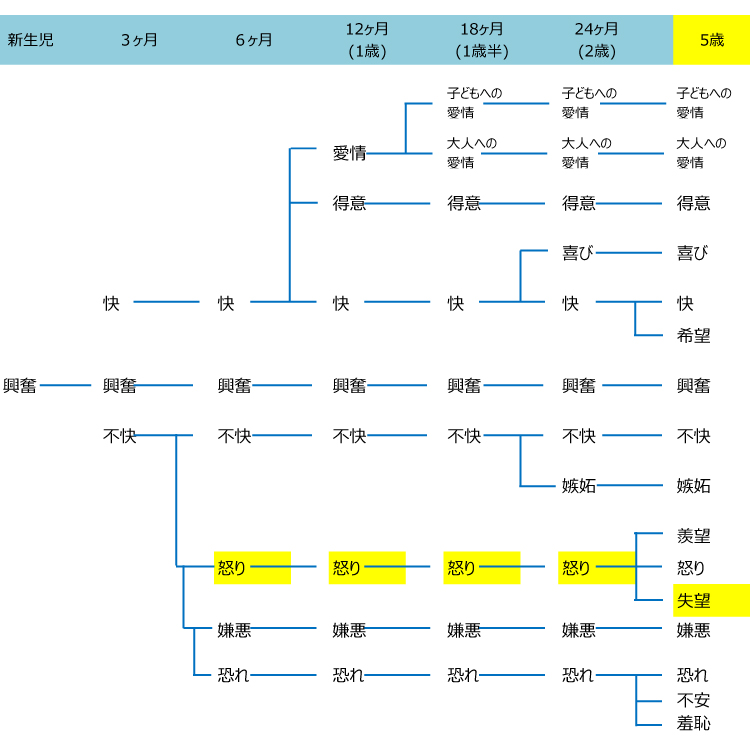
\includegraphics[width=0.6\linewidth,keepaspectratio,bb=0 0 750 750]{fig/fig0_1.jpg}
\caption{ブリッジスの情緒分化図 日本病児保育学会ブログ記事より引用}\label{fig0_1}
\end{figure}

コミュニティの違いによる差異こそあるものの、我々人間の"鳴き声"は言語を為し、その共通認識により対話、伝達が始まったのである。この言語は感情にとどまらず、具象抽象の垣根を超えて叙事や論証、または歌や言葉遊びと言った様々な知的活動の礎となった。動物の鳴き声による対話と対応した人間の会話は、最も原始的な伝達の方法であるものの、様々に技術が発達した今なおコミュニケーションの基礎を為している。通信の始まりは、このような"発話による伝達"であったといえよう。

\subsection{発話の制約}
しかし、単純な発声による発話では、声が届く範囲にしかその意味が届かない。この時の届く範囲とは、空間的な範囲もあれば時間的な範囲でもある。落語会が行われていた会場に、終わった後に入っても落語を聞くことはできないし、また、同じ時間に遠く離れた場所にいても落語を聞くことはできない。肉声の落語を聞くことができるのは、その時その場所で演者と同じ空気を共有していた者に限られる。逆に、その空気を共有している者の中では、選択的に伝えたり聞いたりするということも難しい。高座の上で演者が下座に何らかの指示を出す時、声を使うとすれば客席の幾人かにはどうしても聞こえてしまう。同じ会場で鼾をかいて眠る客がいたとして、これだけを聞かないというのもなかなか無理がある。

先の鼾の例のような雑音があった場合などは特にそうだが、発話によるコミュニケーションでは聞き取れない・追いつかないと言った問題も発生する。マンツーマンのゆっくりした対話であれば言い直してもらえばすむだけの話であるが、先の落語のような例では、そういうわけにも行かない。音自体が聞こえなかった、音は聞こえたけれども判別がつかなかったと言ったレベルから、言語的な問題…イントネーションの差異、語彙にない単語の使用、そもそも言語が異なる、勘違い…と言った知識や思考の問題まで、発話の時には伝達の誤りが起こりうる。

発話による伝達は、原始的であるがゆえに手軽ではあれど制約や問題も内包している。通信・伝達技術というのは、これらの制約や問題を如何に打破するのかという人間の飽くなき挑戦の成果であるとも言える。

\subsection{口伝という方法}
発話の制約を最も単純に外したのは\textbf{口伝}\index{くでん@口伝}である。現在でも民話や民謡など、様々なものが口伝により伝えられているが、これは人間の記憶を介することによって時間や空間の制約を緩和したものといえよう。最も身近なところでは、伝言がそうであろう。もっとも、伝言ゲームに見られる通り、伝達の誤りという問題は解決されているとは言いがたい。「JPCZによる擾乱の影響で山陰地方を中心に荒天となる」などと専門の用語が入った言を伝言したところで、途中に知らぬ人が入れば伝言がうまく行く可能性は低いだろう。また、伝言には意識的・無意識的な取捨選択もあり、伝達の誤りという観点ではむしろ増えているかもしれない。

しかしながら、人間以外の資源が必要ないこの口伝という方法は、最も初期から存在すると同時に、現代まで続いている伝達方法である。口伝の国内における最も古い例としては、稗田阿礼が挙げられる。古事記には彼(彼女?)の誦により伝えられたものが筆録されている。その後の歴史にも、説法や講釈と言った例はほぼ口伝であったようだ。一方、現代で行われている口伝の例としては、先にも持ちだした落語を例に挙げたい。昭和の爆笑王、桂枝雀師は著書「枝雀とヨメはんと七人の弟子」の中で次のように書いておられる。

"一番最初は「ちょっとやるから聞いてなさい」と言って、一字一句口移しで教えることから出発いたします。やらせてみて、ちょっと違うとイントネーションから直す。それが段々お稽古やっていくうちに、五分なら五分、流れを教えるようになる。"

これは、平成のはじめ頃に書かれた文であるし、枝雀師は99年にお隠れになったから、いま他の噺家が同様のやり方をしていると言い切ることはできない。だが、筆者が、この枝雀師の三番弟子、文之助師に"つる"を教わった時は、ほとんどこの通りの教え方であった。ただ、カルチャースクールでのことであるから、録音し、自分で原稿に起こし、その上で直してもらいながらという指導であった。とはいえ、これも口伝には違いない。多くの伝達法がある中で、わざわざこの原始的な口伝という方法で伝承をするのはなぜだろうか。

それは、口伝によってしか伝えられない、空気や情感、発生、身振り手振りの細かな違いなどを伝えられるというところであろう。現代の技術をもってすれば、双方向で似たような指導を遠隔地間で行うことも可能であるように見える。しかし、それでも微妙な空気感や息の間といったものは伝えきれない。落語という芸能は高座の落語家と客席が一体となって作り上げる空間が生命であるから、なるほど、その部分を伝えるためには口伝を取るよりほかないのであろう。また、落語は時代により変化していくものであるから、口伝という形態での変化は逆に追い風となるのであろう。これは、落語の伝承が「ネタの原稿を伝える」のみでないことを示しているといえる。

現代の視点からすれば口伝は古臭く、非効率な手法に見えることも多い。だが、それを意図して取り込んでいる芸に学べる通り、口伝でこそ伝わることもある。通信・伝達技術の多くは、重要と考えにくいものや伝えづらいものを取捨選択しているのである。逆に、その捨てられたものを拾う価値があるシーンや、そこまでの効率を要求しないシーンがあるからこそ、一見古臭く見える通信・伝達の方法も現代に息づいているのである。

\section{書くことによる記録}

口伝は人間の記憶を媒介にして時間や空間の制約を打ち破った。しかしながら、当然全ての人間が稗田阿礼のような記憶力を持つはずもないし、伝達も記憶も個人の状況に依存することとなる。これを打破するのは日本へと輸入された文字であった。

文字とそれを記録する媒体は、ヒエログリフやパピルスと言った著名な例があるとおり古代エジプト文明の時代にまで遡る。楔形文字や漢字と言った様々な文字が青銅器時代に生まれたのである。日本へ文字が入ってくるのは弥生時代とされ、それからの後、8世紀頃には先の稗田阿礼の言を元にした古事記(図\ref{fig0_2})や風土記、日本書紀と言った書物が発行された。

\begin{figure}[htbp]
\centering
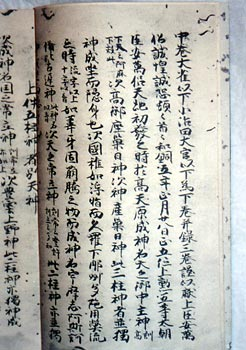
\includegraphics[width=0.6\linewidth,keepaspectratio,bb=0 0 246 350]{fig/fig0_2.jpg}
\caption{真福寺収蔵の国宝・『古事記』 Wikipediaより引用}\label{fig0_2}
\end{figure}

文字の輸入に伴い、離れた場所に文字を書いた媒体を送るという形式での伝送も行われるようになっていった。それらの書物の中には何百年という時を経てなお現代で読むことができるものも多い。これは、文字とその記録媒体が時間と空間の制約を打ち破ったということである。著名な数学者の書簡や日記が見つかることもあれば、伝わるつもり無く詠まれた"この世をば 我が世とぞ思う 望月の 欠けたることも なしと思えば"が現代にまで伝わっている(道長本人は記録に残さなかったが、その場に居合わせた人が日記に記したために現代まで伝わっている)など、文字は言語によって表現可能なものの時間的・空間的制約を打ち破ったのである。汚損や焼失といったリスクこそあるものの、口伝や発話の段階からすれば大きく進歩したと言えるのは明らかであろう。

また、これらの媒体は図画の伝達も可能とした。これは、発話や口伝で伝えられなかったものを伝えられるという利点をもたらした。紙媒体は、文字を媒介に発話を記録すると共に、図画として描けるものも記録する媒体なのである。

\subsection{複写}
書物として残されていく

\subsection{紙媒体が捨てたもの}


\section{遠距離の高速通信:狼煙・手旗信号}


しかし郵便は時間がかかります。ではもっと早く伝えたい場合はどうすればいいかというと、視覚に訴えるものを使えばいいという考えに至りました。

このときに「では煙で通信しよう」となって開発されたのが狼煙です。
また、見える範囲ならば情報をリアルタイムに伝えられる通信として手旗信号といったものも開発されました。

このように口伝から書簡や狼煙、手旗信号に通信の手法を変えることで、遠くに素早く通信できたり、時を越えて通信することができるようになりましたが、言葉にこめられる口調や声の違いといった情報を代わりに失いました。

\section{公開と複製:模写・印刷}

人間は書簡といった文字を記録する媒体を使ううちに、その情報をたくさんの人々に公開するために複製しようと試みるようになりました。

最初は紙に書き写すといった作業だけであったのが、版画で同時に並行して複製ができるようになり、コピー印刷で膨大な量の複製が可能になったりと、時代を重ねるごとに複製の量と質が格段に向上していきました。

\section{通信の秘匿:シーザー暗号・方言での暗号}

ここまでは「広める」通信について考えてきましたが、やはりどうしても人には秘密にしたいことを特定の人に伝えたい場合というときはあるものです。
しかし戦場ではまだ書簡を使って通信していましたが、奪われてしまうといったリスクはどうしても拭いきれませんでした。
このときに情報の秘匿性を高めるために暗号が開発されました。

代表的なものだとシーザー暗号が挙げられます(内容は下記の練習問題を参照)。このような一対一で文字変換を行う暗号を単一換字式暗号と言います。

一方で第二次世界大戦中は薩摩弁が難解であるため暗号として使われたのですが、敵軍の日本人捕虜に傍受した暗号を読ませて平文に変換してしまっていたそうです。
このように暗号としてほとんど意味を成さなかったものも存在します。


\section{記録媒体の変化と増加}

記録媒体というものは時代とともに変化していきます。

ここまでの例だと最初は紙や石版などに文字を書き込むというところから始まり、版画やコピーへと移り変わっていったというようなものです。実際このような移り変わりの中で、記録媒体の数は増加していきました。

では現在使われている記録媒体は昔のどんなものからきたのでしょうか。

\subsection{活動写真という媒体}

活動写真は今の映像の記録媒体の発展に深く関わっている媒体です。
概要としては、観客を呼んで動画を見ながら横で活動弁士と呼ばれる人がその映像について解説する、といったものです。

この活動弁士の音声と活動写真の映像を一緒にしてしまおうと作られたのが映画で、それを映画館などではなく一人で見たいという人のために映画を記録する媒体がビデオテープ、DVD、BDとして開発されました。

このように、活動写真は今の映像記録媒体の発展に大きく役立った存在であると言えます。

\section*{演習問題}
\begin{problems}
\item 歴史的なシーザー暗号では、アルファベットを3文字後ろにずらして(a,d,x,y,zをそれぞれd,g,a,b,cに変えるなど)暗号化していた。1024文字以下1行の半角文字列が入力されるとき、それをシーザー暗号化・復号化するプログラムを作成せよ。
\end{problems}


\part{情報の記録}

\chapter{デジタルデータの記録}

\chapter{アナログデータの記録}

\chapter{情報の圧縮}


\part{電気伝送の方法}

\chapter{電気信号の同期}

\chapter{変調}

\chapter{伝送品質の担保}

\chapter{伝送路の方式}

\chapter{電気通信網の構成}


\part{コンピュータ・ネットワークの基礎}

\chapter{通信プロトコル}

\chapter{コンピュータ・ネットワークの構成}

\chapter{ネットワークアーキテクチャ}

\chapter{ネットワーク機器}

\chapter{Layer1:物理層}

\chapter{Layer2:データリンク層}

\chapter{Layer3:ネットワーク層 (1)IPとアドレス}

\chapter{Layer3:ネットワーク層 (2)ルーティング}

\chapter{Layer4:トランスポート層}

\chapter{Layer5〜7:上位3層}


\part{ネットワーク・プロトコル}

\chapter{ネットワークモデル・再論}

\chapter{telnet}

\chapter{DNS}

\chapter{DHCP}

\chapter{FTP}

\chapter{HTTP}

\chapter{メールに纏わるプロトコル} %SMTP,POP3,IMAP

\chapter{認証に纏わるプロトコル} %Kerberos,LDAP


\part{安定通信網の構築と運用}

\chapter{冗長化}

\chapter{セキュリティ}

\chapter{トラブルシューティング手法の基礎}


%\beginappendix
%\chapter{簡易リファレンス}
%C言語の簡易リファレンスを掲載しておく。紙面の都合上、記述は最小限度にとどめたので、利用方法についてはmanコマンドはじめインターネット等で調べて頂きたい。なお、以下の書籍・サイトを参考にした。
\begin{itemize}
\item C言語によるプログラミング[応用編]第2版(内田他著、Ohm社刊)
\item C言語によるプログラミング[スーパーリファレンス編](内田他著、Ohm社刊)
\item C言語プログラミング(H.M.Deitel他著、ピアソン・エデュケーション刊)
\item プログラミング言語C 第2版 (B.W.Kernighan他著、共立出版刊)
\item Cリファレンスマニュアル第5版(S.P.Harbison他著、SiB access刊)(C99)
\item プログラミング言語Cの新機能(\verb|http://seclan.dll.jp/c99d/|)(C99)
\item C言語関数辞典(\verb|http://www.c-tipsref.com/|)(C99)
\end{itemize}
なお、末尾にC99と付したものはC95,C99で追加された機能について用いたものである。\\

特に断らない限り、大文字で書いているものはマクロであり、型・引数を書いているものは関数である。なお、ヘッダ内で返却値の型や引数の取り方が同じである関数については冒頭にそれを断った上で関数名のみを記している(ctype.hやmath.hなど)。また、便宜上、C89の部分とC95/C99の部分は分けて書き、C95/C99で追加された関数やヘッダはC89の後に追加した。

\section{assert.h(プログラム診断)}
\begin{itemize}
\item \verb|NDEBUG|:定義することで\verb|assert()|を無効にする。
\item \verb|void assert(int expression)|:実行時の条件チェック。\verb|expression|が偽の際にファイル名と行番号を\verb|stderr|に出力して\verb|abort|する。
\end{itemize}
 
\section{ctype.h(文字の分類)}
本ヘッダで定義される関数はいずれも\verb|int function(int argument)|の形である。以下、関数名のみ記している。また、主語「引数が」を省略している。
\begin{itemize}
\begin{multicols}{2}
\item \verb|isalnum|:半角英数字ならば真。
\item \verb|isalpha|:アルファベットならば真。
\item \verb|islower|:英小文字ならば真。
\item \verb|isupper|:英大文字ならば真。
\item \verb|isdigit|:数字ならば真。
\item \verb|isxdigit|:16進数ならば真。
\item \verb|iscntrl|:制御文字ならば真。
\item \verb|ispunct|:区切り文字ならば真。
\item \verb|isspace|:空白文字ならば真。
\end{multicols}
\item \verb|isgraph|:スペース以外の印字可能文字ならば真。
\item \verb|isprint|:スペースを含む印字可能文字ならば真。
\item \verb|tolower|:英大文字であるならば対応する英小文字を返し、それ以外の場合は引数の値を返す。
\item \verb|toupper|:英小文字であるならば対応する英大文字を返し、それ以外の場合は引数の値を返す。
\end{itemize}
以下は、C99において追加された関数である。
\begin{itemize}
\item \verb|isblank|:行中空白ならば真。
\end{itemize}

\section{errno.h(エラー)}
\begin{itemize}
\begin{multicols}{2}
\item \verb|EDOM|:定義域エラー
\item \verb|ERANGE|:値域エラー
\end{multicols}
\item \verb|errno|:エラー状態を保持する外部変数
\end{itemize}

\section{float.h(浮動小数点数型属性検査)}
いずれも環境依存のマクロである。
\begin{itemize}
\item \verb|DBL_DIG|:\verb|double|型変数が10進数で表すことのできる精度の桁数
\item \verb|DBL_EPSILON|:\verb|double|型変数でのマシンイプシロンの値
\item \verb|DBL_MANT_DIG|:\verb|double|型変数の仮数部における基数\verb|FLT_RADIX|の桁数
\item \verb|DBL_MAX|:\verb|double|型変数の表現可能な最大値
\item \verb|DBL_MAX_10_EXP|:\verb|double|型変数の表現可能な指数最大値(基数10)
\item \verb|DBL_MAX_EXP|:\verb|double|型変数の表現可能な指数最大値(基数2)
\item \verb|DBL_MIN|:\verb|double|型変数の表現可能な正の最小値
\item \verb|DBL_MIN_10_EXP|:\verb|double|型変数の表現可能な指数最小値(基数10)
\item \verb|DBL_MIN_EXP|:\verb|double|型変数の表現可能な指数最小値(基数2)
\item \verb|DBL_ROUNDS|:\verb|double|型変数の足し算に対する丸めモード
\item \verb|FLT_DIG|:\verb|float|型変数が10進数で表すことのできる精度の桁数
\item \verb|FLT_EPSILON|:\verb|float|型変数でのマシンイプシロンの値
\item \verb|FLT_MANT_DIG|:\verb|float|型変数の仮数部における基数\verb|FLT_RADIX|の桁数
\item \verb|FLT_MAX|:\verb|float|型変数の表現可能な最大値
\item \verb|FLT_MAX_10_EXP|:\verb|float|型変数の表現可能な指数最大値(基数10)
\item \verb|FLT_MAX_EXP|:\verb|float|型変数の表現可能な指数最大値(基数2)
\item \verb|FLT_MIN|:\verb|float|型変数の表現可能な正の最小値
\item \verb|FLT_MIN_10_EXP|:\verb|float|型変数の表現可能な指数最小値(基数10)
\item \verb|FLT_MIN_EXP|:\verb|float|型変数の表現可能な指数最小値(基数2)
\item \verb|FLT_RADIX|:\verb|float|型変数の指数表現の基数
\item \verb|FLT_ROUNDS|:\verb|float|型変数の足し算に対する丸めモード
\item \verb|LDBL_DIG|:\verb|long double|型変数が10進数で表すことのできる精度の桁数
\item \verb|LDBL_EPSILON|:\verb|long double|型変数でのマシンイプシロンの値
\item \verb|LDBL_MANT_DIG|:\verb|long double|型変数の仮数部における基数\verb|FLT_RADIX|の桁数
\item \verb|LDBL_MAX|:\verb|long double|型変数の表現可能な最大値
\item \verb|LDBL_MAX_10_EXP|:\verb|long double|型変数の表現可能な指数最大値(基数10)
\item \verb|LDBL_MAX_EXP|:\verb|long double|型変数の表現可能な指数最大値(基数2)
\item \verb|LDBL_MIN|:\verb|long double|型変数の表現可能な正の最小値
\item \verb|LDBL_MIN_10_EXP|:\verb|long double|型変数の表現可能な指数最小値(基数10)
\item \verb|LDBL_MIN_EXP|:\verb|long double|型変数の表現可能な指数最小値(基数2)
\item \verb|LDBL_ROUNDS|:\verb|long double|型変数の足し算に対する丸めモード
\end{itemize}
以下はC99において追加されたマクロである。
\begin{itemize}
\item \verb|DECIMAL_DIG|:|:浮動小数点数型で表現できる最大の10進桁数
\item \verb|FLT_EVAL_METHOD|:実際に浮動小数点数演算を行うときの範囲と精度を示す値
\end{itemize}

\section{limits.h(整数型属性検査)}
いずれも環境依存のマクロである。
\begin{itemize}
\item \verb|CHAR_BIT|:\verb|char|型変数のビット数
\item \verb|CHAR_MAX|:\verb|char|型変数の表現可能な最大値
\item \verb|CHAR_MIN|:\verb|char|型変数の表現可能な最小値
\item \verb|INT_MAX|:\verb|int|型変数の表現可能な最大値
\item \verb|INT_MIN|:\verb|int|型変数の表現可能な最小値
\item \verb|LONG_MAX|:\verb|long|型変数の表現可能な最大値
\item \verb|LONG_MIN|:\verb|long|型変数の表現可能な最小値
\item \verb|MB_LEN_MAX|:多バイト文字の最大バイト数
\item \verb|SCHAR_MAX|:\verb|signed char|型変数の表現可能な最大値
\item \verb|SCHAR_MIN|:\verb|signed char|型変数の表現可能な最小値
\item \verb|SHRT_MAX|:\verb|short|型変数の表現可能な最大値
\item \verb|SHRT_MIN|:\verb|short|型変数の表現可能な最小値
\item \verb|UCHAR_MAX|:\verb|unsigned char|型変数の表現可能な最大値
\item \verb|UINT_MAX|:\verb|unsigned int|型変数の表現可能な最大値
\item \verb|ULONG_MAX|:\verb|unsigned long|型変数の表現可能な最大値
\item \verb|USHRT_MAX|:\verb|unsigned short|型変数の表現可能な最大値
\end{itemize}
以下は、C99において追加されたマクロである。
\begin{itemize}
\item \verb|LLONG_MAX|:\verb|long long|型変数の表現可能な最大値
\item \verb|LLONG_MIN|:\verb|long long|型変数の表現可能な最小値
\item \verb|ULLONG_MAX|:\verb|unsigned long long|型変数の表現可能な最大値
\end{itemize}

\section{locale.h(地域情報管理)}
\begin{itemize}
\item \verb|LC_ALL|:全ての地域情報に対する検索・設定用定数
\item \verb|LC_COLLATE|:地域固有の文字の比較順序情報に対する検索・設定用定数
\item \verb|LC_CTYPE|:地域固有文字(多バイト文字等)に対する検索・設定用定数
\item \verb|LC_MONETARY|:地域固有の通貨文字に対する検索・設定用定数
\item \verb|LC_NUMERIC|:地域固有の小数点文字に対する検索・設定用定数
\item \verb|LC_TIME|:地域固有の時間表現文字列に対する検索・設定用定数
\item \verb|NULL|:\verb|NULL|ポインタ
\item \verb|struct lconv|:地域固有の表現情報を格納する構造体
\item \verb|char *setlocale(int category,const char *locale)|:地域情報を設定する。\\ \verb|locale|が\verb|NULL|の時は地域情報を検索する。
\item \verb|struct lconv *localeconv(void)|:地域情報が格納された構造体\verb|lconv|へのポインタを返す。
\end{itemize}

\section{math.h(数学関数)}
gccでコンパイルする際には\verb|-lm|オプションをつけ\verb|gcc source.c -lm|とする必要がある。

以下特に断らない限り、型が省略されたものを\verb|double|型とする。
\begin{itemize}
\item \verb|HUGE_VAL|:\verb|double|型変数の表現可能な最大値(パソコンにおける「十分大きい値」)。C99ではこれにF,Lをつけたものもある。
\begin{multicols}{2}
\item \verb|acos(x)|:逆余弦を返す。$\cos^{-1}(x)$
\item \verb|asin(x)|:逆正弦を返す。$\sin^{-1}(x)$
\item \verb|atan(x)|:逆正接を返す。$\tan^{-1}(x)$
\item \verb|atan2(y,x)|:点$(x,y)$の方向角を返す。$\tan^{-1}(y/x)$。
\item \verb|cos(x)|:余弦を返す。$\cos x$
\item \verb|sin(x)|:正弦を返す。$\sin x$
\item \verb|tan(x)|:正接を返す。$\tan x$
\item \verb|cosh(x)|:双曲余弦を返す。$\cosh x$
\item \verb|sinh(x)|:双曲正弦を返す。$\sinh x$
\item \verb|tanh(x)|:双曲正接を返す。$\tanh x$
\end{multicols}
\item \verb|exp(x)|:引数に対するネイピア数$e=2.718281828\cdots$を底とする指数関数の値を返す。$e^x=\exp x$
\item \verb|frexp(value,int *exp)|:\verb|value|を$x\times 2^t$の形に表し(但し$0.5\le x<1$)、$t$を\verb|*exp|に格納した後、$x$を返す。
\item \verb|ldexp(x,int exp)|:$x\times 2^{\verb|exp|}$を返す。
\item \verb|log(x)|:自然対数を返す。$\ln x=\log_e x$
\item \verb|log10(x)|:常用対数を返す。$\log_{10} x$
\item \verb|modf(value,double* iptr)|:\verb|value|の整数部を\verb|*iptr|に格納したあと、\verb|value|の小数部の値を返す。
\item \verb|pow(x,y)|:$x^y=\exp_x y$の値を返す。
\item \verb|sqrt(x)|:正平方根値$\sqrt{x}$を返す。
\item \verb|ceil(x)|:天井関数値(小数点以下切り上げ値)を返す。$\lceil x \rceil=[x]+1$
\item \verb|floor(x)|:床関数値(小数点以下切り捨て値)を返す。$\lfloor x \rfloor=[x]$
\item \verb|fabs(x)|:絶対値を返す。$|x|$
\item \verb|fmod(x,y)|:$x$の$y$による剰余を返す。
\end{itemize}
C99では大幅に関数・マクロ等が増えた。以下、C99で追加された分である。
\begin{itemize}
\item \verb|INFINITY|:正または符号無しの無限大を示す定数マクロ
\item \verb|NAN|:浮動小数点数型のNANを示す定数マクロ
\item \verb|FP_INFINITE|:正または負の無限大を表すマクロ
\item \verb|FP_NAN|:NANを示すマクロ
\item \verb|FP_NORMAL|:正規化数(正常に表される浮動小数点数)を示すマクロ
\item \verb|FP_SUBNORMAL|:非正規化数(値が小さすぎて正常に表されない浮動小数点数)を示すマクロ
\item \verb|FP_ZERO|:0を表すマクロ
\item \verb|FP_FAST_FMA|:\verb|fma|関数が有意であることを示すマクロで、F,Lをつけたものもある(それぞれ\verb|fmaf,fmal|に対応)
\item \verb|FP_ILOGB0|:\verb|ilogb(0)|の返却値を示すマクロ
\item \verb|FP_ILOGBNAN|:\verb|ilogb(NAN)|の返却値を示すマクロ
\item \verb|MATH_ERRNO|:整数定数1に展開されるマクロ
\item \verb|MATH_ERREXCEPT|:整数定数2に展開されるマクロ
\item \verb|math_errhandling|:\verb|MATH_ERRNO|、\verb|MATH_ERREXCEPT|もしくはこの二つのビット毎論理和に展開されるマクロ
\item \verb|fpclassify(x)|:引数の値をカテゴリに分類する関数マクロ
\item \verb|isfinite(x)|:引数の値が有限の値かどうかを判定する関数マクロ
\item \verb|isinf(x)|:引数の値が無限大かどうかを判定する関数マクロ
\item \verb|isnan|:引数の値が NaN (非数) かどうかを判定する関数マクロ
\item \verb|isnormal(x)|:引数の値が正規化数かどうかを判定する関数マクロ
\item \verb|signbit(x)|:引数の符号が負かどうかを判定する関数マクロ
\item \verb|isgreater(x,y)|:\verb|x|が\verb|y|より大きいかどうかを判定する関数マクロ
\item \verb|isgreaterequal(x,y)|:\verb|x|が\verb|y|より大きい,または等しいかどうかを判定する関数マクロ
\item \verb|isless(x,y)|:\verb|x|が\verb|y|より小さいかどうかを判定する関数マクロ
\item \verb|islessequal(x,y)|:\verb|x|が\verb|y|より小さい,または等しいかどうかを判定する関数マクロ
\item \verb|islessgreater(x,y)|:\verb|x|が\verb|y|より小さい,または大きいかどうかを判定する関数マクロ
\item \verb|isunordered(x,y)|:引数が順序付け可能かどうかを判定する関数マクロ
\item \verb|acosh(x)|:逆双曲線余弦値を返す。$\cosh^{-1}(x)$
\item \verb|asinh(x)|:逆双曲線正弦値を返す。$\sinh^{-1}(x)$
\item \verb|atanh(x)|:逆双曲線正接値を返す。$\tanh^{-1}(x)$
\item \verb|exp2(x)|:引数に対する2を底とする指数関数の値を返す。$2^x=\exp_2 x$
\item \verb|expm1(x)|引数に対して$e^x-1$の値を返す。
\item \verb|log2(x)|:二進対数を返す。$\lg x=\log_2 x$
\item \verb|log1p(x)|:引数に対して$\ln (x+1)$を返す。
\item \verb|logb(x)|:引数の浮動小数点数表現における指数部分を浮動小数点数形式の符号付き整数として返す。
\item \verb|int ilogb(x)|:引数の浮動小数点数表現における指数部分を浮動小数点数形式の符号付き整数として返す。
\item \verb|scalbn(x,int n)|:$x\times$\verb|FLT_RADIX|$^n$を効率よく計算する。\verb|FLT_RADIX|については\\ \verb|float.h|参照。\verb|scalbln|という名前に変えたら、\verb|n|が\verb|long|型になる。
\item \verb|cbrt(x)|:3乗根を返す。$\sqrt[3]{x}$
\item \verb|hypot(x,y)|:過度のオーバーフローやアンダーフローを避けて入力点の原点からの距離を計算する。$\sqrt{x^2+y^2}$
\item \verb|erf(x)|:誤差関数値を返す。$\frac{2}{\sqrt{\pi}}\int^{x}_{0} \exp (-t^2) dt$
\item \verb|erfc(x)|:余誤差関数値を返す。$\frac{2}{\sqrt{\pi}}\int^{\infty}_{x} \exp (-t^2) dt$
\item \verb|tgamma(x)|:ガンマ関数値を返す。$\Gamma(x)=\int^{\infty}_{0} t^{x-1}e^{-t}dt$
\item \verb|lgamma(x)|:引数に対して$\ln|\Gamma(x)|$を返す。
\item \verb|nearbyint(x)|:引数を現在の丸め方向にしたがって浮動小数点数形式の整数値に丸める。例外は発生しない。
\item \verb|rint(x)|:引数を現在の丸め方向にしたがって浮動小数点数形式の整数値に丸める。例外が発生することがある。
\item \verb|long lrint(x)|:引数を現在の丸め方向にしたがって\verb|long|型整数値に丸める。\verb|llrint|とすれば、\verb|long long|型に丸める。
\item \verb|round(x)|:引数を四捨五入する。
\item \verb|long lround(x)|:引数を四捨五入して\verb|long|型にする。\verb|llround|とすれば、\verb|long long|型にする。
\item \verb|trunc(x)|:絶対値の小数点以下を切り捨てて返す。
\item \verb|remainder(x,y)|:IEEE60559規格に則った剰余を返す。\verb|remquo|も同様。
\item \verb|copysign(x,y)|:$x$の絶対値と$y$の符号を持った値を返す。$\frac{y}{|y|}|x|$
\item \verb|nan(const char *p)|:文字列をNaNに変換する。
\item \verb|nextafter(x,y)|:$y$方向に見たとき、$x$の次に表現可能な数値を返却する。\verb|nexttoword|関数はこの第2引数が\verb|long double|になったもの。
\item \verb|fmax(x,y)|:二つの引数のうち大きい方の値を返す。
\item \verb|fmin(x,y)|:二つの引数のうち小さい方の値を返す。
\item \verb|fdim(x,y)|:$x>y$なら$x-y$を、そうでなければ0を返す。
\item \verb|fma(x,y,z)|:$x\times y+z$を返却する。
\end{itemize}
また、ここには記さないが、C99では上記に挙げた関数の関数名終端に\verb|f|を付すと関数・引数とも\verb|float|型に、\verb|l|を付すと\verb|long double|型になる(\verb|double|以外で特記しているものを除く)。C99では\verb|math.h|も\verb|complex.h|も含め、\verb|tgmath.h|をインクルードすることで\verb|math.h|の\verb|double|型関数名で関数が使えるようになる。

\section{setjmp.h(非局所分岐)}
\begin{itemize}
\item \verb|jmp_buf|:\verb|longjmp|時に必要な環境を格納するための配列型
\item \verb|void longjmp(jmp_buf env,int val)|:\verb|env|に格納した環境を復元して\verb|setjmp|の位置に戻る(第2引数は\verb|setjmp|の返却値)。
\item \verb|int setjmp(jmp_buf env)|:\verb|longjmp|時のための環境を\verb|env|に格納する。
\end{itemize}

\section{signal.h(シグナル処理)}
\begin{itemize}
\item \verb|sig_atomic_t|:シグナルを保持する変数の型
\item \verb|SIG_DFL|:シグナルに対して処理系のデフォルトの処理を指示するマクロ
\item \verb|SIG_ERR|:シグナルの設定失敗を示すマクロ
\item \verb|SIG_IGN|:シグナルを無視することを示すマクロ
\begin{multicols}{2}
\item \verb|SIGABRT|:異常終了
\item \verb|SIGFPE|:算術演算エラー
\item \verb|SIGILL|:不正命令
\item \verb|SIGINT|:非同期割り込み
\item \verb|SIGSEGV|:メモリの不正アクセス
\item \verb|SIGTERM|:プログラム終了
\end{multicols}
\item \verb|(*signal(int sig,void(*func)(int)))(int)|:シグナル(\verb|sig|)が発生した際の処理関数設定。返却値は成功時その関数へのポインタ、失敗時\verb|SIG_ERR|。
\item \verb|int raise(int sig)|:シグナル(\verb|sig|)を発生させる。成功時は0,失敗時は非0を返す。
\end{itemize}

\section{stdarg.h(可変引数)}
\begin{itemize}
\item \verb|va_list|:可変引数リストを扱う変数の型
\item \verb|type va_arg(va_list ap,type)|:可変引数リスト\verb|ap|より\verb|type|で示す引数を返す。
\item \verb|void va_end(va_list ap)|:可変引数リスト\verb|ap|を処理して終了させる。
\item \verb|void va_start(va_list ap,parmN)|:\verb|parmN|の次から始まる可変引数リスト\verb|ap|の初期化を行う。
\end{itemize}
以下はC99で追加された関数である。
\begin{itemize}
\item \verb|void va_copy(va_list dst, va_list src)|:\verb|va_start|で\verb|va_list|を初期化したオブジェクト\verb|src|のコピー\verb|dst|を作成する。
\end{itemize}

\section{stddef.h(共通定義)}
\begin{itemize}
\item \verb|NULL|:\verb|NULL|ポインタ
\item \verb|ptrdiff_t|:2つのポインタの差を表現する型
\item \verb|size_t|:\verb|sizeof|演算子の返す符号なし整数型
\item \verb|wchar_t|:\verb|wide|文字の型
\item \verb|offsetof(type,member-designator)|:構造体\verb|type|内での構造体メンバ\\ \verb|member-designator|のオフセットを返す。
\end{itemize}

\section{stdio.h(標準入出力)}
以下、特に断らない限り、\verb|stream|は\verb|FILE *stream|を示し、ストリームポインタとする。
\begin{itemize}
\item \verb|FILE|:ファイルストリーム格納変数型
\item \verb|fpos_t|:ファイル内の位置を表す型
\item \verb|size_t|:\verb|sizeof|演算子の返す符号なし整数型
\item \verb|_IOFBF|:フルバッファリングでストリーム入出力を行う(\verb|setvbuf|の\verb|mode|)
\item \verb|_IOLBF|:ラインバッファリングでストリーム入出力を行う(\verb|setvbuf|の\verb|mode|)
\item \verb|_IONBF|:バッファリングせずにストリーム入出力を行う(\verb|setvbuf|の\verb|mode|)
\item \verb|BUFSIZ|:\verb|setbuf|で使用するバッファサイズ
\item \verb|EOF|:ファイル終端
\item \verb|FILENAME_MAX|:ファイル名の最大長
\item \verb|FOPEN_MAX|:同時オープン可能ファイル個数
\item \verb|L_tmpnam|:\verb|tmpnam|でつくられる一時ファイル名の最大長
\item \verb|TMP_MAX|:\verb|tmpnam|で作ることができる一時ファイルの最大個数
\begin{multicols}{2}
\item \verb|NULL|:\verb|NULL|ポインタ
\item \verb|SEEK_CUR|:現在のファイル位置指示
\item \verb|SEEK_END|:ファイルの最後
\item \verb|SEEK_SET|:ファイルの先頭
\item \verb|stdin|:標準入力ストリーム
\item \verb|stdout|:標準出力ストリーム
\end{multicols}
\item \verb|stderr|:標準エラー出力ストリーム
\item \verb|int remove(const char *fn)|:\verb|fn|の示すファイルを削除する。
\item \verb|int rename(const char *old,const char *new)|:\verb|old|で示すファイル名を\verb|new|で示すファイル名に変更する。
\item \verb|FILE *tmpfile(void)|:一時ファイルを作成してそのファイルストリームを返す。
\item \verb|char *tmpnam(char *s)|:一意な一時ファイル名を生成して\verb|s|に格納し、その名前を関数値として返す。
\item \verb|int fclose(stream)|:引数のストリームをクローズする。
\item \verb|int fflush(stream)|:引数のストリームをフラッシュする。
\item \verb|FILE *fopen(const char *fn,const char *mode)|:\verb|mode|に従って\verb|fn|の示すファイルをオープンしてストリームを返す。
\item \verb|FILE *freopen(const char *fn,const char *mode,stream)|:\verb|mode|に従って\verb|fn|の示すファイルを再オープンして\verb|stream|にストリームを返す。
\item \verb|void setbuf(stream,char *buf)|:\verb|stream|のバッファリングをバッファ\verb|buf|を用いて行う。
\item \verb|int setvbuf(stream,char *buf,int mode,size_t size)|:\verb|stream|のバッ\\ファリングをバッファ\verb|buf|を用いて\verb|mode,size|に従って行う。
\item \verb|int fprintf(stream,const char *format,...)|:\verb|format|に従い\verb|stream|にデータを出力する。
\item \verb|int fscanf(stream,const char *format,...)|:\verb|format|に従い\verb|stream|からデータを入力する。
\item \verb|int printf(const char *format,...)|:\verb|format|に従い\verb|stdout|にデータを出力する。
\item \verb|int scanf(const char *format,...)|:\verb|format|に従い\verb|stdin|からデータを入力する。
\item \verb|int sprintf(char *s,const char *format,...)|:\verb|format|に従ってデータを文字列\verb|s|に出力する。
\item \verb|int sscanf(char *s,const char *format,...)|:\verb|format|に従ってデータを文字列\verb|s|から入力する。
\item \verb|int vfprintf(stream,const char *format,va_list arg)|:\verb|format|に従い\\ \verb|stream|に可変引数リスト\verb|arg|の内容を出力する。
\item \verb|int vprintf(const char *format,va_list arg)|:\verb|format|に従い\verb|stdout|に可変引数リスト\verb|arg|の内容を出力する。
\item \verb|int vsprintf(char *s,const char *format,va_list arg)|:\verb|format|に従い文字列\verb|s|に可変引数リスト\verb|arg|の内容を出力する。
\item \verb|int fgetc(stream)|:\verb|stream|より1文字入力してその文字を返す。
\item \verb|char *fgets(char *s,int n,stream)|:\verb|stream|より\verb|n|文字入力して\verb|s|に格納し、\verb|s|へのポインタを返す。
\item \verb|int fputc(int c,stream)|:\verb|c|を\verb|stream|に出力する。
\item \verb|int fputs(const char *s,stream)|:\verb|s|を\verb|stream|に出力する。
\item \verb|int getc(stream)|:\verb|stream|より1文字入力してその文字を返す。
\item \verb|int getchar(void)|:\verb|stdin|より1文字入力してその文字を返す。
\item \verb|char *gets(char *s)|:\verb|stdin|より1行入力して\verb|s|に格納し、\verb|s|へのポインタを返す(改行コードが\verb|NULL|文字に置き換えられる)。
\item \verb|int putc(int c,stream)|:\verb|c|を\verb|stream|に出力する。
\item \verb|int putchar(int int c)|:\verb|stdout|に\verb|c|を出力して\verb|c|を返す。
\item \verb|int puts(const char *s)|:\verb|s|を\verb|stdout|に出力する。(\verb|NULL|文字が抜かれて改行コードが補われる。)
\item \verb|int ungetc(int c,stream)|:\verb|stream|に\verb|c|を戻し、\verb|c|を返す。
\item \verb|size_t fread(void *ptr,size_t size,size_t nmemb,stream)|:\\ \verb|stream|から\verb|size|分のデータ\verb|nmemb|個を入力して\verb|ptr|にセットする。
\item \verb|size_t fwrite(const void *ptr,size_t size,size_t nmemb,stream)|:\\ \verb|stream|に\verb|size|分のデータ\verb|nmemb|個を\verb|ptr|から出力する。
\item \verb|int fgetpos(stream,fpos_t *pos)|:\verb|stream|のファイル位置指示子の値を求めて\verb|pos|にセットする。
\item \verb|int fseek(stream,long int offset,int whence)|:\verb|stream|に対しファイル位置\\ \verb|whence|と移動量\verb|offset|を変更する。
\item \verb|int fsetpos(stream,fpos_t *pos)|:\verb|stream|のファイル位置を\verb|pos|に変更する。
\item \verb|long int ftell(stream)|:引数のファイルポジションインジケータの値を返す。
\item \verb|void rewind(stream)|:引数のファイルポジションインジケータをファイル先頭にセットする。
\item \verb|void clearerr(stream)|:引数の\verb|EOF|及びエラー指示子をクリアする。
\item \verb|int feof(stream)|:引数のファイル終端指示子を調べ、\verb|EOF|ならば非0を返す。
\item \verb|int ferror(stream)|:引数のエラー状態指示子を調べ、エラーならば非0を返す。
\item \verb|void perror(const char *s)|:\verb|errno|に対応するエラーメッセージを\verb|stderr|に出力する。
\end{itemize}
以下はC99において追加された関数である。
\begin{itemize}
\item \verb|int snprintf(char *s,size_t n,const char *format,...)|:\verb|format|に従ってデータを\verb|n|文字分、文字列\verb|s|に出力する。返却値は出力文字数。
\item \verb|int vsnprintf(char *s,size_t n,const char *format,va_list arg)|\\:\verb|format|に従い文字列\verb|s|に\verb|n|文字分可変引数リスト\verb|arg|の内容を出力する。返却値は出力文字数。
\item \verb|int vscanf(const char *format,va_list arg)|:\verb|scanf|の可変個数引数部分を可変引数リスト\verb|va_list|に変更したもの。
\item \verb|int vsscanf(const char *s,const char *format,va_list arg)|:\verb|sscanf|の可変個数引数部分を\verb|va_list|に変更したもの。
\item \verb|int vfscanf(stream,const char *format,va_list arg)|:\verb|fscanf|の可変個数引数部分を\verb|va_list|に変更したもの。
\end{itemize}

\section{stdlib.h(ユーティリティ)}
以下特に断らない限り、\verb|n|及び\verb|size|は\verb|size_t|型とし、\verb|str|は\verb|const char *|型とする。
\begin{itemize}
\item \verb|div_t|:\verb|div()|の返す型
\item \verb|ldiv_t|:\verb|ldiv()|の返す型
\item \verb|size_t|:\verb|sizeof|演算子の返す符号なし整数型
\item \verb|wchar_t|:\verb|wide|文字の型
\item \verb|EXIT_FAILURE|:プログラムの実行が失敗したことを示す
\item \verb|EXIT_SUCCESS|:プログラムの実行が成功したことを示す
\item \verb|MB_CUR_MAX|:その時点でのマルチバイト文字を表現するのに必要な最大バイト数
\item \verb|NULL|:\verb|NULL|ポインタ
\item \verb|RAND_MAX|:疑似乱数の最大値
\item \verb|double atof(str)|:\verb|str|を浮動小数点数に変換して返す。
\item \verb|int atoi(str)|:\verb|str|を整数に変換して返す。
\item \verb|long int atol(str)|:\verb|str|を\verb|long|型整数にして返す。
\item \verb|double strtod(str,char **endptr)|:\verb|str|を浮動小数点数に変換し(先頭の空白文字はスキップされる)、浮動小数点より後ろの文字列へのポインタを\verb|*endptr|に格納する。返却値は変換された浮動小数点数。
\item \verb|long int strtol(str,char **endptr,int base)|:\verb|str|を\verb|base|によって指定された記数法にしたがって\verb|long|型に変換し(先頭の空白文字はスキップされる)、その数値より後ろの文字列へのポインタを\verb|*endptr|に格納する。返却値は変換された数。
\item \verb|unsigned long int strtoul(str,char **endptr,int base)|:\verb|str|を\verb|base|によって指定された記数法にしたがって\verb|unsigned long|型に変換し(先頭の空白文字はスキップされる)、その数値より後ろの文字列へのポインタを\verb|*endptr|に格納する。返却値は変換された数。
\item \verb|int rand(void)|:0から\verb|RAND_MAX|の範囲で疑似乱数を発生させ、その値を返す。
\item \verb|void srand(unsigned int seed)|:引数を疑似乱数発生ルーチンの種として与える。
\item \verb|void *calloc(n,size)|:\verb|size|バイト\verb|n|個分の動的メモリを割り当て、それを0クリアする。
\item \verb|void free(voind *ptr)|:引数のポインタで与えられた動的メモリ領域を解放する。
\item \verb|void *malloc(size)|:\verb|size|バイト分の動的メモリを割り当てる。
\item \verb|void *realloc(void *ptr,size)|:\verb|ptr|で示される動的メモリを\verb|size|バイト分の大きさで再割り当てする。
\item \verb|void abort(void)|:プログラムを異常終了する。
\item \verb|int atexit(void (*func)(void))|:プログラム終了時に実行する関数を登録する。
\item \verb|void exit(int status)|:引数を返却値としてプログラムを終了する。
\item \verb|char *getenv(str)|:環境変数\verb|str|に対応する文字列へのポインタを返す。
\item \verb|int system(str)|:\verb|str|に示されるプログラム(コマンドライン形式)を実行する。
\item \begin{verbatim}
void *bsearch(const void *key,const void *base,n,size,
  int (*compare)(const void *, const void *))
\end{verbatim}:配列(\verb|base|、要素毎のサイズ\verb|size|、要素数\verb|n|)内のデータ中のキー\verb|key|に一致するデータをバイナリサーチで検索し、その要素へのポインタを返す。比較は\verb|compare|で示される比較関数によって行う。
\item \begin{verbatim}
void qsort(void *base,n,size,
  int (*compare)(const void *, const void *))
\end{verbatim}:配列(\verb|base|、要素毎のサイズ\verb|size|、要素数\verb|n|)を\verb|compare|で示される比較関数に従ってソートする。
\item \verb|int abs(int j)|:整数引数の絶対値を返す。
\item \verb|long int labs(long int j)|:\verb|long|型引数の絶対値を返す。
\item \verb|div_t div(int num,int denom)|:\verb|num|/\verb|denom|の商と剰余を\verb|div_t|型で返す。
\item \verb|ldiv_t ldiv(long int num,long int denom)|:\verb|num|/\verb|denom|の\\商と剰余を\verb|ldiv_t|型で返す。
\item \verb|int mblen(str,n)|:マルチバイト文字列\verb|str|を最大\verb|n|バイトまで検査して、次のマルチバイト文字のバイト数を返す。
\item \verb|int mbtowc(wchar_t *pwc,str,n)|:マルチバイト文字\verb|str|を最初から\verb|n|バイトまで\verb|wide|文字(\verb|pwc|)に変換する。
\item \verb|int wctomb(char *s,wchar_t wchar)|:\verb|wide|文字(\verb|wchar|)をマルチバイト文字\verb|s|に変換する。
\item \verb|size_t mbstowcs(wchar_t *pwcs,str,n)|:マルチバイト文字列\verb|str|を最初から\verb|n|バイトまで\verb|wide|文字列(\verb|pwcs|)に変換する。
\item \verb|size_t wcstombs(char *s,const wchar_t *pwcs,n)|:\verb|wide|文字列(\verb|pwcs|)を最初から\verb|n|バイトまでマルチバイト文字列\verb|s|に変換する。
\end{itemize}
以下はC99において追加された型/関数である。
\begin{itemize}
\item \verb|lldiv_t|:\verb|lldiv()|の返す型
\item \verb|void _Exit(int status)|:プログラムを正常終了する。
\item \verb|float strtof(str,char **endp)|:\verb|strtod|の\verb|float|版
\item \verb|long double strtold(str,char **endp)|:\verb|strtod|の\verb|long double|版
\item \verb|long long int strtoll(str,char **endptr,int base)|:\verb|strtol|の\\ \verb|long long int|版
\item \verb|unsigned long long int strtoull(str,char **endptr,int base)|:\verb|strtol|の\\ \verb|unsigned long long int|版
\item \verb|long long int atoll(str)|:\verb|atoi|の\verb|long long int|版
\item \verb|long long int llabs(long long int j)|:\verb|abs|の\verb|long long int|版
\item \verb|lldiv_t lldiv(long long int num,long long int denom)|:\verb|ldiv|の\\ \verb|long long int|版
\end{itemize}

\section{string.h(文字列操作)}
以下特に断らない限り、\verb|s1|,\verb|s2|,\verb|s|はいずれも\verb|char *|型とし、\verb|m1|,\verb|m2|,\verb|m|は\verb|void *|型とする。但し、\verb|const s2|等と書いた場合は、\verb|const char *|型等、前に\verb|const|を付すものとする。また、\verb|n|は\verb|size_t|型とする。
\begin{itemize}
\item \verb|size_t|:\verb|sizeof|演算子の返す符号なし整数型
\item \verb|NULL|:\verb|NULL|ポインタ
\item \verb|void *memcpy(m1,const m2,n)|:\verb|m2|を\verb|m1|に\verb|n|バイト分コピーする。
\item \verb|void *memmove(m1,const m2,n)|:\verb|m2|を\verb|m1|に\verb|n|バイト分コピーする。(\verb|m2|と\verb|m1|が重なっても良い。)
\item \verb|int memcmp(const m1,const m2,n)|:\verb|m1|,\verb|m2|を\verb|n|バイトまで比較し、一致したら0,一致しなければ非0を返す。
\item \verb|void *memchr(const m,int c,n)|:文字\verb|c|を\verb|m|の最初の\verb|n|バイト中から探し、あればその文字へのポインタを、なければ\verb|NULL|を返す。
\item \verb|void *memset(m,int c,n)|:\verb|m|を文字\verb|c|で\verb|n|バイト分埋める。
\item \verb|char *strcpy(s1,const s2)|:\verb|s1|に\verb|s2|をコピーする。
\item \verb|char *strncpy(s1,const s2,n)|:\verb|s1|に\verb|s2|を最大\verb|n|バイトまでコピーする。
\item \verb|char *strcat(s1,const s2)|:\verb|s1|の後ろに\verb|s2|を連結する。
\item \verb|char *strncat(s1,const s2,n)|:\verb|s1|の後ろに\verb|s2|を最大\verb|n|バイトまで連結する。
\item \verb|int strcmp(const s1,const s2)|:\verb|s1|,\verb|s2|を比較し、一致したら0,一致しなければ非0を返す。
\item \verb|int strcoll(const s1,const s2)|:地域情報を使い\verb|s1|,\verb|s2|を比較し、一致したら0,一致しなければ非0を返す。
\item \verb|int strncmp(const s1,const s2,n)|:\verb|s1|,\verb|s2|を\verb|n|バイトまで比較し、一致したら0,一致しなければ非0を返す。
\item \verb|size_t strxfrm(s1,const s2,n)|:\verb|s2|を地域情報にしたがって\verb|s1|に最初の\verb|n|バイトだけ変換する。
\item \verb|char *strchr(const s,int c)|:文字\verb|c|を\verb|s|中から探し、あればその文字へのポインタを、なければ\verb|NULL|を返す。
\item \verb|size_t strcspn(const s1,const s2)|:\verb|s2|に含まれない文字だけで構成される文字列を\verb|s1|から探し、その最初の部分の長さを返す。
\item \verb|char *strpbrk(const s1,const s2)|:\verb|s2|中の文字が\verb|s1|に出てくる、その最初の文字へのポインタを返す。
\item \verb|char *strrchr(const s,int c)|:\verb|s|中で文字\verb|c|が現れる最後の位置のポインタを返す。
\item \verb|size_t strspn(const s1,const s2)|:\verb|s2|に含まれる文字だけで構成される文字列を\verb|s1|から探し、その最初の部分の長さを返す。
\item \verb|char *strstr(s)|:\verb|s2|が\verb|s1|に出てくる最初の文字へのポインタを返す。
\item \verb|char *strtok(s1,const s2)|:\verb|s1|を区切り記号文字列\verb|s2|にしたがってトークンに分割する。\verb|s1|は2回目以降の呼び出しにおいて\verb|NULL|を指定する。トークンがあればそのポインタを,なければ\verb|NULL|を返す。
\item \verb|char *strerror(int errnum)|:エラー番号\verb|errnum|を文字列に変換し、そのポインタを返す。
\item \verb|size_t strlen(const s)|:\verb|s|の長さを返す。
\end{itemize}

\section{time.h(時間)}
\begin{itemize}
\item \verb|clock_t|:\verb|clock()|の返却値の型
\item \verb|time_t|:カレンダ時間の型
\item \verb|size_t|:\verb|sizeof|演算子の返す符号なし整数型
\item \verb|CLOCKS_PER_SEC|:\verb|clock_t|における1秒間の数
\item \verb|NULL|:\verb|NULL|ポインタ
\item \verb|clock_t clock(void)|プログラムの実行に要した経過時間を返す。
\item \verb|double difftime(time_t time1,time_t time2)|:\verb|time1|と\verb|time2|の差を秒で返す。
\item \verb|time_t mktime(struct tm *timeptr)|:ローカル時間\verb|timeptr|をカレンダ時間に変換して返す。
\item \verb|time_t time(time_t *timer)|:現在のカレンダ時間を\verb|timer|にセットし、カレンダ時間を返す。
\item \verb|char *asctime(const struct tm *timeptr)|:ローカル時間\verb|timeptr|を文字列に変換して返す。
\item \verb|char *ctime(const time_t *timer)|:カレンダ時間\verb|timer|を文字列に変換して返す。
\item \verb|struct tm *gmtime(const time_t *timer)|:カレンダ時間\verb|timer|を世界標準時に変換して返す。
\item \verb|struct tm *localtime(const time_t *timer)|:カレンダ時間\verb|timer|をローカル時間に変換して返す。
\item \begin{verbatim}
size_t strftime(char *s,size_t max,
  const char *fm,const struct tm *tptr)
\end{verbatim}:ローカル時間\verb|tptr|を表示形式\verb|fm|に従い、最大\verb|max|文字まで変換し、\verb|s|にセットする。
\end{itemize}

\section{iso646.h(代替綴・C95)}
本ヘッダはC95において追加されたヘッダである。演算子をマクロを用いて記すためのヘッダであり、以下はいずれもマクロである。
\begin{multicols}{2}
\begin{itemize}
\item \verb|and|:置き換える演算子は\verb|&&|
\item \verb|and_eq|:置き換える演算子は\verb|&=|
\item \verb|bitand|:置き換える演算子は\verb|&|
\item \verb|bitor|:置き換える演算子は$|$
\item \verb|compl|:置き換える演算子は\verb|~|
\item \verb|not|:置き換える演算子は\verb|!|
\item \verb|not_eq|:置き換える演算子は\verb|!=|
\item \verb|or|:置き換える演算子は$||$
\item \verb|or_eq|:置き換える演算子は$|=$
\item \verb|xor|:置き換える演算子は\verb|^|
\item \verb|xor_eq|:置き換える演算子は\verb|^=|
\end{itemize}
\end{multicols}

\section{wchar.h(ワイド文字・C95)}
本ヘッダはC95において追加されたヘッダである。ひとまず、型とマクロを記す。
\begin{itemize}
\item \verb|wchar_t|:\verb|wide|文字の型
\item \verb|wint_t|:\verb|wchar_t|に加えて、拡張文字で表示されない値をひとつ以上示す広義整数型
\item \verb|mbstate_t|:マルチバイト文字からワイド文字への変換状態を示す型
\item \verb|size_t|:\verb|sizeof|演算子の返す符号なし整数型
\item \verb|NULL|:\verb|NULL|ポインタ
\item \verb|WCHAR_MIN|:\verb|wchar_t|型の最小値
\item \verb|WCHAR_MAX|:\verb|wchar_t|型の最大値
\item \verb|WEOF|:ファイル終端を示す\verb|wint_t|型の値
\end{itemize}
次いで、他のヘッダの関数と直接には対応しない関数を示す。\verb|c_(型)|は\verb|const (型)|を示す。
\begin{itemize}
\item \verb|fwide(FILE *stream,int mode)|:\verb|stream|の入出力単位を\verb|mode|が負の場合はバイト単位、正の場合はワイド文字単位に設定する。0の場合は設定を変更しない。\verb|mode|と同符号の値を返却する。
\item \verb|wint_t btowc(int c)|:引数の1バイト文字をワイド文字に変換して返す。
\item \verb|int wctob(wint_t c)|:引数のワイド文字を1バイト文字に変換して返す。
\item \verb|int mbsinit(c_mbstate_t *ps)|:引数の\verb|mbstate_t|オブジェクトが初期変換状態を表すかどうかを判定し、表す場合は非0、表さない場合は0を返す。
\item \verb|size_t mbrlen(c_char *s,size_t n,mbstate_t *ps)|:マルチバイト文字のバイト長を取得する。
\item \verb|size_t mbrtowc(wchar_t *c,c_char *s, size_t n,mbstate_t *ps)|:変換状態格納領域を\verb|ps|とし、マルチバイト文字をワイド文字に変換する。
\item \verb|size_t wcrtomb(char *s,wchar_t wc,mbstate_t *ps)|:変換状態格納領域を\verb|ps|とし、ワイド文字をマルチバイト文字に変換する。
\item \verb|size_t mbsrtowcs(wchar_t *p,c_char **s, size_t n,mbstate_t *ps)|:変換状態格納領域を\verb|ps|とし、\verb|s|の示すマルチバイト文字列を\verb|n|バイト分ワイド文字列に変換して\verb|p|に格納する。返却値はエラーが出れば-1、処理成功時は変換に成功したヌル文字以外の文字の数である。
\item \verb|size_t wcsrtombs(char *s,c_wchar_t **src,size_t n,mbstate_t *ps)|:変換状態格納領域を\verb|ps|とし、\verb|src|の示すワイド文字列を\verb|n|バイト分マルチバイト文字列に変換して\verb|s|に格納する。返却値はエラーが出れば-1、処理成功時は変換に成功したヌル文字以外の文字の数である。
\end{itemize}
以下に示す関数は\verb|stdio.h|,\verb|stdlib.h|等の関数の\verb|char|の部分を\verb|wchar_t|に変更したものである。それ故、型や引数は省き、対応する関数を挙げておく。
\begin{multicols}{2}
\begin{itemize}
\item \verb|fwprintf|:\verb|fprintf|に対応
\item \verb|fwscanf|:\verb|fscanf|に対応
\item \verb|swprintf|:\verb|snprintf|に対応
\item \verb|swscanf|:\verb|sscanf|に対応
\item \verb|vfwprintf|:\verb|vfprintf|に対応
\item \verb|vswprintf|:\verb|vsprintf|に対応
\item \verb|vwprintf|:\verb|vprintf|に対応
\item \verb|wprintf|:\verb|printf|に対応
\item \verb|wscanf|:\verb|scanf|に対応
\item \verb|fgetwc|:\verb|fgetc|に対応
\item \verb|fgetws|:\verb|fgets|に対応
\item \verb|fputwc|:\verb|fputc|に対応
\item \verb|fputws|:\verb|fputs|に対応
\item \verb|getwc|:\verb|getc|に対応
\item \verb|getwchar|:\verb|getchar|に対応
\item \verb|putwc|:\verb|putc|に対応
\item \verb|putwchar|:\verb|putchar|に対応
\item \verb|ungetwc|:\verb|ungetc|に対応
\item \verb|wcstod|:\verb|strtod|に対応
\item \verb|wcstol|:\verb|strtol|に対応
\item \verb|wcstoul|:\verb|strtoul|に対応
\item \verb|wcscpy|:\verb|strcpy|に対応
\item \verb|wcsncpy|:\verb|strncpy|に対応
\item \verb|wmemcpy|:\verb|memcpy|に対応
\item \verb|wmemmove|:\verb|memmove|に対応
\item \verb|wcscat|:\verb|strcat|に対応
\item \verb|wcsncat|:\verb|strncat|に対応
\item \verb|wcscmp|:\verb|strcmp|に対応
\item \verb|wcscoll|:\verb|strcoll|に対応
\item \verb|wcsncmp|:\verb|strncmp|に対応
\item \verb|wcsxfrm|:\verb|strxfrm|に対応
\item \verb|wmemcmp|:\verb|memcmp|に対応
\item \verb|wcschr|:\verb|strchr|に対応
\item \verb|wcscspn|:\verb|strcspn|に対応
\item \verb|wcspbrk|:\verb|strpbrk|に対応
\item \verb|wcsrchr|:\verb|strrchr|に対応
\item \verb|wcsspn|:\verb|strspn|に対応
\item \verb|wcsstr|:\verb|strstr|に対応
\item \verb|wcstok|:\verb|strtoken|に対応
\item \verb|wmemchr|:\verb|memchr|に対応
\item \verb|wcslen|:\verb|strlen|に対応
\item \verb|wmemset|:\verb|memset|に対応
\item \verb|wcsftime|:\verb|strftime|に対応
\end{itemize}
\end{multicols}
以下は、C99において追加された関数である。
\begin{multicols}{2}
\begin{itemize}
\item \verb|wcstoull|:\verb|strtoull|に対応
\item \verb|wcstoll|:\verb|strtoll|に対応
\item \verb|wcstof|:\verb|strtof|に対応
\item \verb|wcstold|:\verb|strtold|に対応
\item \verb|vwscanf|:\verb|vscanf|に対応
\item \verb|vswscanf|:\verb|vsscanf|に対応
\item \verb|vfwscanf|:\verb|vfscanf|に対応
\end{itemize}
\end{multicols}

\section{wctype.h(ワイド文字変換・C95)}
本ヘッダはC95において追加されたヘッダである。まず、型とマクロを示す。
\begin{itemize}
\item \verb|wctype_t|:ワイド文字の種別を表す型
\item \verb|wctrans_t|:あるワイド文字を他のワイド文字に変換できるマッピングを表現する型
\item \verb|wint_t|:\verb|wchar_t|に加えて、拡張文字で表示されない値をひとつ以上示す広義整数型
\item \verb|WEOF|:ファイル終端を示す\verb|wint_t|型の値
\end{itemize}
他のヘッダの関数と対応のない関数は以下の通り。
\begin{itemize}
\item \verb|int iswctype(wint_t wc,wctype_t desc)|:\verb|wc|が\verb|desc|に属するワイド文字か否か判定し、属する場合は非0を、属さない場合は0を返す。
\item \verb|wint_t towctrans(wint_t wc,wctrans_t desc)|:\verb|desc|の変換に従って\verb|wc|を変換して返却する。
\item \verb|wctrans_t wctrans(const char *p)|:\verb|p|によって識別される変換の値を返却する。
\item \verb|wctype_t wctype(const char *p)|:\verb|p|によって識別されるワイド文字の種別を返却する。
\end{itemize}
上記以外は対応する関数が\verb|ctype.h|にある。対応する関数の引数の型を\verb|wint_t|に変更したものが本ヘッダ内の関数である。
\begin{multicols}{2}
\begin{itemize}
\item \verb|iswalnum|:\verb|isalnum|に対応
\item \verb|iswalpha|:\verb|isalpha|に対応
\item \verb|iswcntrl|:\verb|iscntrl|に対応
\item \verb|iswdigit|:\verb|isdigit|に対応
\item \verb|iswgraph|:\verb|isgraph|に対応
\item \verb|iswlower|:\verb|islower|に対応
\item \verb|iswprint|:\verb|isprint|に対応
\item \verb|iswpunct|:\verb|ispunct|に対応
\item \verb|iswspace|:\verb|isspace|に対応
\item \verb|iswupper|:\verb|isupper|に対応
\item \verb|iswxdigit|:\verb|isxdigit|に対応
\item \verb|towlower|:\verb|tolower|に対応
\item \verb|towupper|:\verb|toupper|に対応
\end{itemize}
\end{multicols}
以下は、C99において追加された関数である。
\begin{itemize}
\item \verb|iswblank|:\verb|isblank|に対応
\end{itemize}

\section{complex.h(複素数演算・C99)}
本ヘッダはC99において追加されたヘッダである。まず、マクロを掲載しておく。
\begin{itemize}
\item \verb|complex|:型名\verb|_Complex|を表す
\item \verb|_Complex_I|:\verb|const float _Complex|型の虚数単位
\item \verb|imaginary|:型名\verb|_Imaginary|を表す
\item \verb|_Imaginary_I|:\verb|const float _Imaginary|型の虚数単位
\item \verb|I|:虚数単位(型は環境依存)
\end{itemize}
本ヘッダ内の関数は\verb|math.h|に対応した関数のあるものが多い。以下にそれを挙げておく。なお、関数の型・引数の型とも、特記しないものは\verb|double complex|型とする。
\begin{multicols}{2}
\begin{itemize}
\item \verb|cacos(z)|:\verb|acos|に対応
\item \verb|casin(z)|:\verb|asin|に対応
\item \verb|catan(z)|:\verb|atan|に対応
\item \verb|ccos(z)|:\verb|cos|に対応
\item \verb|csin(z)|:\verb|sin|に対応
\item \verb|ctan(z)|:\verb|tan|に対応
\item \verb|ccosh(z)|:\verb|cosh|に対応
\item \verb|csinh(z)|:\verb|sinh|に対応
\item \verb|ctanh(z)|:\verb|tanh|に対応
\item \verb|cacosh(z)|:\verb|acosh|に対応
\item \verb|casinh(z)|:\verb|asinh|に対応
\item \verb|catanh(z)|:\verb|atanh|に対応
\item \verb|cexp(z)|:\verb|exp|に対応
\item \verb|clog(z)|:\verb|log|に対応
\item \verb|cpow(x,y)|:\verb|pow|に対応
\item \verb|csqrt(z)|:\verb|sqrt|に対応
\item \verb|double cabs(z)|:\verb|fabs|に対応
\end{itemize}
\end{multicols}
以下は複素数特有の関数である。
\begin{multicols}{2}
\begin{itemize}
\item \verb|conj(z)|:共役複素数を返す。$\overline{z}$
\item \verb|cproj(z)|:リーマン球面上への射影値を返す。
\item \verb|double cart(z)|:仰角を返す。
\item \verb|double creal(z)|:実部を返す。
\item \verb|double cimag(z)|:虚部を返す。
\end{itemize}
\end{multicols}
本ヘッダも\verb|math.h|同様、上記に挙げた関数の関数名終端に\verb|f|を付すと関数・引数とも\verb|float complex|型に、\verb|l|を付すと\verb|long double complex|型になる(\verb|double|以外で特記しているものを除く)。また、\verb|math.h|も\verb|complex.h|も含め、\verb|tgmath.h|をインクルードすることで\verb|math.h|の\verb|double|型関数名(複素数に特有の関数は\verb|complex.h|の\verb|double complex|型関数名)で関数が使えるようになる。

\section{fenv.h(浮動小数点数環境・C99)}
本ヘッダはC99において追加されたヘッダである。
\begin{itemize}
\item \verb|fenv_t|:現在の浮動小数点数環境情報を格納する型
\item \verb|fexcept|:例外に関する情報を格納する型
\begin{multicols}{2}
\item \verb|FE_DIVBYZERO|:ゼロ除算例外
\item \verb|FE_INEXACT|:不正確例外
\item \verb|FE_INVALID|:不正操作例外
\item \verb|FE_OVERFLOW|:オーバーフロー例外
\item \verb|FE_UNDERFLOW|:アンダーフロー例外
\item \verb|FE_ALL_EXCEPT|:処理系定義の全例外
\item \verb|FE_DOWNWARD|:$-\infty$の方向へ丸める
\item \verb|FE_TONEAREST|:最も近い値へ丸める
\item \verb|FE_TOWARDZERO|:0方向へ丸める
\item \verb|FE_UPWARD|:$+\infty$の方向へ丸める
\item \verb|FE_DFL_ENV|:デフォルトの浮動小数点数環境
\end{multicols}
\item \verb|int fegetexceptflag(fexcept_t *f, int e)|:\verb|e|で指定された例外フラグを実装定義依存の値として\verb|f|に格納する。もし格納に成功した場合には0を、失敗した場合には、非0を返す。
\item \verb|int fesetexceptflag(const fexcept_t *f, int e)|:\verb|f|で指定されたオブジェクトでの表現に従い、\verb|e|で指定された例外フラグに対する完全な状態をセットする。\verb|e|が0か状態の設定に成功した場合には0を返す。それ以外は非0を返す。この関数ではフラグの状態をセットするだけで例外は発生しない。
\item \verb|int feclearexcept(int e)|:\verb|e|で指定された例外フラグのクリアを試みる。\verb|e|が0かクリアが成功した場合に0を返す。それ以外は非0を返す。
\item \verb|int fetestexcept(int e)|:\verb|e|で指定された例外フラグが現在セットされているか検査し、セットされている例外フラグ値を返す。
\item \verb|int feraiseexcept(int e)|:\verb|e|で指定された例外を発生させる。\verb|e|が0か例外の発生に成功した場合は0を返す。それ以外は非0を返す。
\item \verb|int fegetround(void)|:現在の丸めモードを丸めフラグの値で返す。 
\item \verb|int fesetround(int r)|:\verb|r|で指定された丸めモードにセットする。引数が丸めフラグの値でないときは状態は変更されない。引数で指定された丸め方向に設定できたときに限り0を返す。 
\item \verb|int fegetenv(fenv_t *e)|:現在の浮動小数点数環境を\verb|e|に格納する。成功すると0を返す。 
\item \verb|int fesetenv(const fenv_t *e)|:現在の浮動小数点数環境に指定された浮動小数点数環境\verb|e|を設定する。設定に成功すると0を返す。 
\item \verb|int feholdexcept(fenv_t *e)|:現在の浮動小数点数環境を\verb|e|に格納し、例外フラグをクリアし、可能であれば全例外に対し(例外でも継続する)非停止モードに設定する。もし非停止モードに設定できたときは0を返す。 
\item \verb|int feupdateenv(const fenv_t *e)|:現在発生した例外を一時領域に格納し、\verb|e|で指定された浮動小数点数環境を設定した後、一時領域に格納した例外を発生させる。例外発生に成功した場合には0を返す。 
\end{itemize}

\section{inttypes.h(整数型書式・C99)}
本ヘッダはC99において追加されたヘッダである。書式設定用マクロについては本文参照。ここでは対応関数を示すに留める。
\begin{multicols}{2}
\begin{itemize}
\item \verb|imaxabs|:\verb|abs|の\verb|intmax_t|版
\item \verb|imaxdiv|:\verb|div|の\verb|intmax_t|版
\item \verb|strtoimax|:\verb|strtol|の\verb|intmax_t|版
\item \verb|strtoumax|:\verb|strtol|の\verb|uintmax_t|版
\item \verb|wcstoimax|:\verb|wcstol|の\verb|intmax_t|版
\item \verb|wcstoumax|:\verb|wcstol|の\verb|uintmax_t|版
\end{itemize}
\end{multicols}

\section{stdbool.h(論理・C99)}
本ヘッダはC99において追加されたヘッダである。マクロのみのヘッダである。
\begin{itemize}
\item \verb|bool|:\verb|_Bool|型を示す
\item \verb|true|:整数定数1に展開する
\item \verb|false|:整数定数0に展開する
\item \verb|__bool_true_false_are_defined|:整数定数1に展開する
\end{itemize}

\section{stdint.h(整数型管理・C99)}
本ヘッダはC99において追加されたヘッダである。マクロのみのヘッダである。なお、マクロ中の\verb|N|には通常、8,16,32,64の何れかが入り、これが幅指定となる。
\begin{itemize}
\item \verb|INTN_MIN|:幅指定符号付き整数型の最小値
\item \verb|INTN_MAX|:幅指定符号付き整数型の最大値
\item \verb|UINTN_MAX|:幅指定符号無し整数型の最大値
\item \verb|INT_LEASTN_MIN|:最小幅指定符号付き整数型の最小値
\item \verb|INT_LEASTN_MAX|:最小幅指定符号付き整数型の最大値
\item \verb|UINT_LEASTN_MAX|:最小幅指定符号無し整数型の最大値
\item \verb|INT_FASTN_MIN|:最速最小幅指定符号付き整数型の最小値
\item \verb|INT_FASTN_MAX|:最速最小幅指定符号付き整数型の最大値
\item \verb|UINT_FASTN_MAX|:最速最小幅指定符号無し整数型の最大値
\item \verb|INTPTR_MIN|:ポインタ保持可能な符号付き整数型の最小値
\item \verb|INTPTR_MAX|:ポインタ保持可能な符号付き整数型の最大値
\item \verb|UINTPTR_MAX|:ポインタ保持可能な符号付き整数型の最大値
\item \verb|INTMAX_MIN|:最大幅符号付き整数型の最小値
\item \verb|INTMAX_MAX|:最大幅符号付き整数型の最大値
\item \verb|UINTMAX_MAX|:最大幅符号無し整数型の最大値
\item \verb|PTRDIFF_MIN|:\verb|ptrdiff_t|の限界値下限
\item \verb|PTRDIFF_MAX|:\verb|ptrdiff_t|の限界値上限
\item \verb|SIG_ATOMIC_MIN|:\verb|sig_atomic_t|の限界値下限
\item \verb|SIG_ATOMIC_MAX|:\verb|sig_atomic_t|の限界値上限
\item \verb|SIZE_MAX|:\verb|size_t|の限界値
\item \verb|WCHAR_MIN|:\verb|wchar_t|の限界値下限
\item \verb|WCHAR_MAX|:\verb|wchar_t|の限界値上限
\item \verb|WINT_MIN|:\verb|wint_t|の限界値下限
\item \verb|WINT_MAX|:\verb|wint_t|の限界値上限
\item \verb|INTN_C(値)|:値を\verb|int_leastN_t|に対応する整数定数式に展開
\item \verb|UINTN_C(値)|:値を\verb|uint_leastN_t|に対応する整数定数式に展開
\item \verb|INTMAX_C(値)|:値を\verb|intmax_t|である整数定数式に展開
\item \verb|UINTMAX_C(値)|:値を\verb|uintmax_t|である整数定数式に展開
\end{itemize}

\section{tgmath.h(型総称数学関数・C99)}
本ヘッダはC99において追加されたヘッダである。このヘッダの中の関数マクロはmath.hあるいはcomplex.hのdoubleの関数と同名である。引数の型によって関数を使い分けるのがこのヘッダの目的である。詳細は本文を参照されたい。

\newpage


%\chapter{一部解説の付記}
%\input{AppendixB}

%\chapter{Cに関連したWebサービス}
%\input{AppendixC}

%\chapter*{参考書籍等紹介}
%本書を読む上で、あるいは読まれた後で参考となる書籍・サイトを紹介しておく。なお、参考となる書籍/サイトはこの他にも多数あるが、ここでは目についたものを紹介するにとどめた。実際には、学習者自身の目で本・サイトを選ばれたい。

\subsection*{文法の解説}
\begin{itemize}
 \item C言語プログラミング(H.M.ダイテル/P.J.ダイテル著 小嶋隆一訳・ピアソンエデュケーション):現在出ているCの文法書籍の中で、最も練習問題が多いもののひとつ。説明もなかなかわかり易く、内容も浅くない。
 \item C実践プログラミング(S.オウアルライン著  望月康司監訳・オライリージャパン):上記ダイテルに比べてやや難しめであるが、内容に妥協のないCの文法書。
 \item 美しいCプログラミング見本帖(柏原正三著・翔泳社):C言語の難所「ポインタ」の観点から、「習うより慣れろ」の精神で文法を見ていく好著。ポインタのみを書いている書籍よりも広い視点でCを学ぶことができる。
 \item 本当は怖いC言語(種田元樹著・秀和システム):本書同様、C言語を理論的に説明した好著。エラーを出すプログラムを掲載し、それにより学ぶなど随所に工夫が見られる。C99にも対応している。
 \item 苦しんで覚えるC言語(\url{http://9cguide.appspot.com/}):私の知る限り最も丁寧な解説サイト。Windowsでの環境構築から全て書いてあり、非常にわかりやすい説明が行われている。最近書籍版が出た。
 \item 目指せプログラマー(\url{http://www5c.biglobe.ne.jp/~ecb/index.html}|):C言語を始め幾つかの言語と、アルゴリズム論の基礎を解説しているサイト。
 \item Programming Place Plus(\url{http://www.geocities.jp/ky_webid/index.html}):他に見られない項目も含めて細かくCを解説しているサイト。
\end{itemize}

\subsection*{Cリファレンス}
\begin{itemize}
 \item Cリファレンスマニュアル 第5版(S.P.ハービソン/G.L.スティールJr.著 玉井浩訳・SIBアクセス):現在出ているCの辞書では最も充実しているもののひとつ。
 \item C言語によるプログラミングスーパーリファレンス編(内田智史他著・オーム社):初心者向けのCの辞書だが、1999年のCの改定に対応していないのが難点。
\end{itemize}

\subsection*{その他、参考になる本}
\begin{itemize}
 \item プログラミング言語C第2版(カーニハン,リッチー著 石田晴久訳・共立出版):C言語の原典である書籍。
 \item エキスパートCプログラミング(P.リンデン著 梅原系訳・アスキー):C言語の内容についてかなり深く突っ込んだ書籍。
 \item C/C++の「迷信」と「誤解」(高木信尚著・技術評論社):非常に細かい、勘違いしやすい場所について仕様を基に突っ込んでいく書籍。
 \item 補講C言語(平田豊著・工学社):入門書では余り触れられない実践テクニックを紹介する書籍。
 \item C言語によるはじめてのアルゴリズム入門(河西朝雄著・技術評論社):アルゴリズムについて、C言語で、簡単なものを中心に紹介した好著。
 \item C言語による最新アルゴリズム事典(奥村晴彦著・技術評論社):「最新」ではなくなってきたが、C言語を用いて多くのアルゴリズムが書かれている。
 \item アルゴリズム演習300題(橋本英美著・日刊工業新聞社):簡単な問題を中心としたプログラミングの演習書。初歩的な問題も掲載されており、練習に調度良い。
 \item 演習でマスターするC言語とデータ構造(内藤広志,斉藤隆著・共立出版):データ構造と派生型について1冊通して演習する書籍。
 \item プログラマのための論理パズル(D.E.シャシャ著 吉平健治訳・オーム社):プログラミングに必要な様々な発想をパズルを元に学ぶ書籍。アルゴリズムの能力を上げるのに役立つ。
 \item Short Coding(Ozy著・毎日コミュニケーションズ):C言語で「できる限り短いソースを書く」ことに視点を当てて書かれた書籍。この書籍を楽しむことでC言語やアルゴリズムへの深い理解を得ることができる。お遊びの本といえばそうなのであるが、驚くほど有用である。
 \item プログラミングコンテストチャレンジブック(秋葉拓哉他著・毎日コミュニケーションズ):競技プログラミングに焦点を当てたプログラミングの書籍。
 \item ニューメリカル・レシピ・イン・シー(W.H.プレス他著 奥村晴彦他訳・技術評論社):数値計算に関する、標準的な参考書。
 \item ロベールのC++入門講座(ロベール著・毎日コミュニケーションズ):C++の入門書であるが、前半5章はCにも共通する部分であり、非常に良い解説が行われている。引き続きC++を学ぶ気があるならば推奨する。ページ数の割に安い。
 \item ストラウストラップのプログラミング入門(B.ストラウストラップ著 遠藤美代子訳・翔泳社):C++を作った人が書いた、プログラミング全般をC++を用いて入門するという内容の書。
\end{itemize}


%\chapter*{おわりに}
%「お疲れ様でした!」本書を読み終えられた人に、まずはそう申し上げたい。同時に、構想から1年以上をかけ、ようやくテキストを書き終えた自分にも同じ言葉を贈りたい。
\\ \\ 
近年、「C言語は古びた言語であるから、学ぶ価値がない」というような論調を見聞する。たしかに、C++やJavaなどのより強力な言語があるし、LLも数多く出ている現在、Cを実践で使う機会は減ってきているのかも知れない。だが、私は「C言語を一度学ぶことはどの言語を主で使うにしても有用である」と思う。これは例えば、英文学を考えてみればわかるだろう。シェイクスピアの作品は古典と言われる部類に属するだろうが、非常に豊かな語彙をはじめとして、現代から見ても決して読む価値のないものではない。それどころか、シェイクスピアを知らないことは無教養とさえされているところがある。我が国で言えば、明治から大正にかけての文学は、たしかに古いものであるが、そこから学ぶところは決して少なくないだろう。
\\ \\ 
この様な重要な古典としてC言語を捉えた時、多くの言語に影響を与えていることがわかる。C言語を学ぶことは、現代よく用いられる言語の背景にある考えを理解することである。科学を見ても歴史を見ても、背景の考えを理解することが有用なのは言うまでもないことであろう。
\\ \\ 
これらの「背景の考え」を初心者のうちから理解していれば、他の言語の学習も捗る。この考えから、本書は「C言語の文法を中心に、背景の考えをよく理解できる説明」を行うようにしたつもりである。それがどの程度達成されているかは読者諸賢の判断を待つしかないが…。
\\ \\ 
本書は、理論の面からプログラミングの楽しさを伝えようとしてみたものであるが、果たして上手く伝えることができただろうか。その答えは、読者の皆様がこれからプログラミングに携わっていく中で自ずと見えてくることだろう。もしも本書を読むことによってプログラミング好きが一人でも増えたのであれば、本書の目的は達成されたといえるだろう。
\\ \\ 
本テキストを利用してくれた人たち、本テキストの執筆に携わってくれた全ての人たちに心よりの感謝を捧げ、筆を置くことにする。
\begin{flushright}
中島みゆき「ローリング」を聞きながら\\
達哉ん
\end{flushright}



\printindex

\end{document}
